\section{Расчёт параметров и составление принципиальной электрической схемы}

\subsection{Схема включения ОУ}
Схема включения К154УД4 (HA2520) приведена на рис. \ref{fig:opamp-topology}, а также в табл. \ref{tab:opamp-topology}.
Имеется подстроечный резистор, осуществляющий балансировку ''0'' ОУ, т.к. $f_н \ne 0$.
\begin{figure}[!ht]
    \centering
    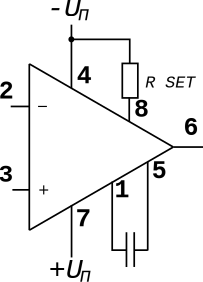
\includegraphics[width=0.4\linewidth]{opamp-topology.pdf}
    \caption{Схема включения К154УД4 (HA2520)}
    \label{fig:opamp-topology}
\end{figure}

\begin{table}[!ht]
    \centering
    \caption{Назначение выводов К154УД4 (HA2520)}
    \label{tab:opamp-topology}
    \begin{tabular}{|c|c|}
        \hline
        Вывод & Назначение \\ \hline
        1     & Не используется \\ \hline
        2     & Инвертирующий вход \\ \hline
        3     & Неинвертирующий вход \\ \hline
        4     & Отрицательное напряжение питания \\ \hline
        5     & Частотная коррекция \\ \hline
        6     & Выход \\ \hline
        7     & Положительное напряжение питания \\ \hline
        8     & Корпус \\ \hline
    \end{tabular}
\end{table}

\subsection{Выбор резисторов цепи ООС}
Проектируемое устройство "--- прецизионный масштабный, т.е. высокоточный, усилитель, поэтому резисторы следует выбирать так же прецизионные, т.е. такие, что их допуск равен $\delta R \sim (0.05 \div 0.1)~\%$.
Наиболее подходящей будет серия Р1-37 "--- это металлодиэлектрические изолированные резисторы.
Так как по техническому заданию $P_{пот} \le 1~Вт$, то необходимо выбрать резистор с номинальной мощностью рассеяния не меньше этой величины.
В обозначенной выше серии, таким условиям удовлетворяет вид Р1-37-0602 с номинальной мощностью рассеяния равной $P_{рас} = 125~мВт$ и диапазоном сопротивлений $(10\==100 \cdot 10^3)~Ом$.
Для данного в техническом задании температурного диапазона устройство будет иметь допуск $\delta R = 0.05~\%$, уровень собственных шумов достаточно мал и достигает 1~мкВ/В, $ТКС = \pm10 \cdot 10^{-6}~\degree C^{-1}$ для температур от $20~\degree C$ и $ТКС = \pm50 \cdot 10^{-6}~\degree C^{-1}$ для температур от $-60~\degree C$ до $+20~\degree C$.
Далее будем использовать последнее значение.

По техническому заданию сопротивление $R_{вх} \ge 0.1~кОм$.
Будем считать его достаточно низким, следовательно использовать можно схему включения инвертирующего усилителя на входе.

Остальные каскады целесообразно включать также по схеме инвертирующего усилителя по следующим причинам:
\begin{itemize}
    \item в них отсутствует погрешность усиления от синфазноо сигнала;
    \item в усилителях переменного тока инвертирующий усилитель содержит меньшее число резисторов и имеет малое значени $U_{ош.вых}$ (постоянное напряжение на выходе ОУ при отсутствии входного сигнала);
    \item в промежуточных каскадах не требуется большого входного сопротивления.
\end{itemize}

Коэффициент усиления инвертирующего усилителя при идеальном ОУ определяется по формуле
\[
    K = -\frac{R_2}{R_1}.
\]

Исходя из этого и принимая коэффициент усиления каждого каскада $K = 31.62$, выбираем следующие номиналы резисторов:
\begin{itemize}
    \item $R_1 = 3.16~кОм$, $R_2 = 100~кОм$ "--- резисторы в цепи обратной связи первого каскада;
    \item $R_3 = 3.16~кОм$, $R_4 = 100~кОм$ "--- резисторы в цепи обратной связи второго каскада;
\end{itemize}

\subsection{Погрешность коэффициента усиления}
Коэффициенты усиления, рассчитанные ранее, соответствуют идеальному усилителю, в реальном же, естественно, будет сказываться влияние некоторых характеристик, считаемых ранее идеальными.

Один из основных неидеальных параметров "--- коэффициент усиления, который (как и входное сопротивление) в реальном случае не бесконечен.
Погрешность выражается как
\[
    \epsilon_к = \frac{\frac{R_2}{R_1} + \frac{R_2}{R_{вх}}}{K R_{НЭ}} (R_{вых} + R_{НЭ}),
\]
% TODO: Разобраться
%где $R_{НЭ} \approx R_н \parallel (R_1 + R_2) = \frac{2 \cdot (3.16 + 100)}{2 + (3.16 + 100)} = 1.96$ "--- эквивалентное сопротивление нагрузки, $R_{вых}$ "--- выходное сопротивление ОУ.
где $R_{НЭ} \approx R_н \parallel (R_1 + R_2)$ "--- эквивалентное сопротивление нагрузки, $R_{вых}$ "--- выходное сопротивление ОУ.
Учитывая, что второе сопротивление гораздо больше первого, а сопротивление нагрузки "--- это либо входное сопротивление следующего каскада, либо сопротивление нагрузки усилителя, получаем погрешности усиления каждого каскада порядка ${\epsilon_к}_i = 0.018~\%$, а всего усилителя $\epsilon = 0.036~\%$.

Кроме погрешностей, обусловленных неидеальностью параметров ОУ возникает погрешность за счёт разброса значений резисторов в цепи ООС, равная $\epsilon_R = \delta R_2 - \delta R_1$.

Были выбраны прецизионные резисторы, по этой причине данная погрешность достаточно мала $\epsilon_R = (\pm0.05 \pm 0.05)~\% = \pm0.1~\%$.

В процессе эксплуатации коэффициент усиления ПУ может меняться из-за влияния температуры окружающей среды.
Температурная нестабильность коэффициента усиления $\epsilon_{TK}$ вызвана в основном изменением коэффициента усиления ОУ и номиналов резисторов $R_1$ и $R_2$ и определяется по формуле
\[
    \epsilon_{TK} = \frac{\delta K}{1 + \frac{K}{K_{ИД}}},
\]
где $\delta K$ "--- относительное изменение коэффициента усиления в заданном диапазоне температур.

Исходя из условий технического задания определим $\epsilon_{TK}$:
\[
    {\epsilon_{TK}}_i
    = \frac{\pm35~\%}{1 + \frac{10000}{10}}
    \approx \pm0.105~\%.
\]

Окончательно для всех каскадов в целом получаем:
\[
    \epsilon_{TK}
    = {\epsilon_{TK}}_1 + {\epsilon_{TK}}_2 + {\epsilon_{TK}}_3
    = 0.315~\%.
\]

Определим погрешность из-за температурной нестабильности резисторов:
\[
    \epsilon_{RT}
    = (ТКС_2 - ТКС_1) \cdot \Delta T_{\max} \cdot 100~\%
    = (\pm50 \pm 50) \cdot 10^{-6} \cdot 35 \cdot 100~\%
    = \pm0.350~\%,
\]
где $\Delta T_{\max} = \frac{1}{2} (T_{\max} - T_{\min})$ "--- максимальное отклонение температуры от медианного значения.

Окончательно для всех каскадов в целом получаем:
\[
    \epsilon_{RT}
    = {\epsilon_{RT}}_1 + {\epsilon_{RT}}_2 + {\epsilon_{RT}}_3
    = 1.075~\%.
\]

Тогда суммарная погрешность составляет
\[
    \epsilon
    = \epsilon_K + \epsilon_R + \epsilon_{TK} + \epsilon_{RT}
    % = (0.036 + 0.1 + 0.315 + 0.1050)~\%
    = 1.501~\%.
\]

\subsection{Влияние напряжения смещения нуля и входных токов}
При отсутствии входного сигнала на выходе ОУ появляется постоянное напряжение $U_{ош.вых}$.
Рассчитаем $U_{ош.вых}$ для первого каскада:
\[
    {U_{ош.вых}}_1
    = U_{см} + I_{вх} R_2
    = 6 \cdot 10^{-3} + 10 \cdot 10^{-9} \cdot 100 \cdot 10^3
    \approx 7~мВ.
\]

При отсутствии разделительного конденсатора для второго каскада эта величина будет складываться из собственного $U_{ош.вых}$ второго каскада и усиленного $U_{ош.вых}$ первого каскада:
\[
    {U_{ош.вых}}_2
    = U_{см} + K \cdot {U_{ош.вых}}_1
    = 6 \cdot 10^{-3} + 31.62 \cdot 7 \cdot 10^{-3}
    \approx 227~мВ.
\]
Эта величина достаточно мала, учитывая, что питание составляет $U_п = 15~В$.
Необходимо поставить разделительные конденсаторы на вход и выход всего усилителя.

\subsection{Расчёт разделительных конденсаторов}
Ёмкость $C$ разделительного конденсатора следует выбирать, исходя из ограничений на коэффициент частотных искажений, появляющихся на низких частотах.

% \[
%     M_1
%     = \sqrt{1 + \left(\frac{1}{2 \pi \tau_н f_н}\right)^2},
% \]
% где $\tau_н = (R_{вых.пр} + R_{вх.посл}) \cdot C$ "--- постоянная времени RC-цепи, образованной разделительным конденсатором, входным сопротивлем предыдущего каскада $R_{вых.пр}$ и входным сопротивлением последующего каскада $R_{вх.посл}$.
\[
    M_н
    = 10^\frac{M_{н}~[Дб]}{20}
    = 10^\frac{0.15~Дб}{20}
    \approx 1.017,
\]
откуда принимая, что $R_г << R_{вх}$ получаем
\[
    C
    = \frac{1}{2 \pi f_н (R_г + R_{вх}) \sqrt{M_н^2 - 1}}
    = \frac{1}{2 \pi \cdot 100 \cdot 3.16 \cdot 10^3 \cdot \sqrt{1.017^2 - 1}}
    \approx 2.72~мкФ.
\]

\subsection{Устранение паразитной положительной обратной связи через источник питания}
% \begin{figure}[!h]
%     \centering
%     \includegraphics[width=0.5\textwidth]{alone-amplifier}
%     \caption{Принципиальная схема каскада проектируемого усилителя}
%     \label{alone-amplifier}
% \end{figure}
За счёт источника питания может появляться паразитная положительная обратная связь (ППОС), которая будет плохо влиять на режим работы операционных усилителей.
Чтобы нейтрализовать влияние ППОС через источник питания на выводы операционного усилителя можно поставить RC-фильтры.

Величины элементов $R_3$, $R_4$ (соединены первым каскадом), $R_7$, $R_8$ (соединены вторым каскадом), выбираются из соображений, что падение напряжения питания на резисторах не должно превышать одного вольта ($\Delta U_п << U_п = 15~В$)

Тогда
\[
    R_3 = R_4 = R_7 = R_8
    = \frac{\Delta U}{I_{пот}}
    = \frac{1}{8 \cdot 10^{-3}}
    = 125~Ом.
\]

\begin{figure}[!ht]
    \centering
    \includegraphics[width=\textwidth]{amplifier.pdf}
    \caption{Принципиальная схема проектируемого усилителя}
    \label{amplifier}
\end{figure}

Проведём моделирование собранной схемы (рис. \ref{fig:oscillogram-sine} и \ref{fig:oscillogram-impulse}).
АЧХ усилителя изображён на рис. \ref{fig:frequency-response-lower} и \ref{fig:frequency-response-high}.

% \begin{figure}[!h]
%     \centering
%     \begin{subfigure}[b]
%         \centering
%         \includegraphics[width=0.4\textwidth]{oscillogram-sine}
%         \caption{}
%         % \caption{Моделирование при гармоническом сигнале: масштаб на канале A равен 5~мВ/дел; на канале B "--- 5~В/дел}
%         % \label{fig:oscillogram-sine}
%     \end{subfigure}
%     \begin{subfigure}[b]
%         \centering
%         \includegraphics[width=0.4\textwidth]{oscillogram-impulse}
%         \caption{}
%         % \caption{Моделирование при импульсном сигнале: масштаб на канале A равен 5~мВ/дел; на канале B "--- 5~В/дел}
%         % \label{fig:oscillogram-impulse}
%     \end{subfigure}
%     \caption{Моделирование а) при гармоническом сигнале: масштаб на канале A равен 5~мВ/дел; на канале B "--- 5~В/дел}; при б) импульсном сигнале: масштаб на канале A равен 5~мВ/дел; на канале B "--- 5~В/дел}
%     \label{fig:oscillogram}
% \end{figure}

\begin{figure}[!ht]
    \centering
    \includegraphics[width=0.8\textwidth]{oscillogram-sine}
    \caption{Моделирование при гармоническом сигнале: масштаб на канале A равен 5~мВ/дел; на канале B "--- 5~В/дел}
    \label{fig:oscillogram-sine}
\end{figure}

\begin{figure}[!ht]
    \centering
    \includegraphics[width=0.8\textwidth]{oscillogram-impulse}
    \caption{Моделирование при импульсном сигнале: масштаб на канале A равен 5~мВ/дел; на канале B "--- 5~В/дел}
    \label{fig:oscillogram-impulse}
\end{figure}

\begin{figure}[!h]
    \centering
    \includegraphics[width=0.8\textwidth]{frequency-response-lower}
    \caption{АЧХ моделируемого усилителя, маркер на нижней частоте}
    \label{fig:frequency-response-lower}
\end{figure}

\begin{figure}[!h]
    \centering
    \includegraphics[width=0.8\textwidth]{frequency-response-high}
    \caption{АЧХ моделируемого усилителя, маркер на верхней частоте}
    \label{fig:frequency-response-high}
\end{figure}

Из рис. \ref{fig:frequency-response-lower} и \ref{fig:frequency-response-high} видно, что реализованная схема прецизионного усилителя обеспечивает стабильное усиление на заданном диапазоне частот от 100~Гц до 100~кГц.
